\section{Implications for Distributed Systems}

\subsection{Space is simply time}

Dedalus programs can model many classes of distributed systems.  Consider the (distributed) dedalus program

\begin{Dedalus}
ping(@A, B)@(A, B, N) \(\leftarrow\)
  init(A, @B)@N; 

pong(@B, A)@r(A, B, N) \(\leftarrow\)
  ping(@A, B)@N;
\end{Dedalus}

And its rewrite in Datalog$\lnot$ with choice:

\begin{Dedalus}
ping(A, B, S) \(\leftarrow\)
  init(A, B, N),
  successor(N, S),
  choose((_), (S));

pong(B, A, S) \(\leftarrow\)
  ping(A, B, N),
  successor(N, S),
  choose((_), (S));
  
\end{Dedalus}

We may regard  \emph{r()} as a function over the attributes occurring in the body of the rule.  \wrm{I still think that time and the head predicate need to be inputs to r(), to ensure that duplicate facts are derived at the same time, and there are no implicit timing dependencies between facts in different predicates with the same key values.} The implementation or \emph{r()} is provided by
the model.  For example:

\subsubsection{Synchronous Systems}

r(\_) = 1 for all \_.  Computation proceeds in rounds.

\subsubsection{Asynchronous Systems}

The return value of r may be any arbitrary integer, positive or negative, including a NULL integer indicating an infinite value.

\subsubsection{Lamport Clocks}

As a middle ground, we might wish to enforce a constraint that $r(\_) > 0$.  Doing so would entail implementing a \emph{Lamport Clock}. 

\paa{part of me is considering dispensing with this r() stuff.  call it ``later", and define it in terms of choice over successor.  then the above enumeration
of ``implementations of $r$" becomes an enumeration of selection conditions to add to each ``later" rule}

\subsubsection{Synchronous Systems2}

We enforce that $S = N + 1$.

\subsubsection{Asynchronous Systems2}

%%The return value of r may be any arbitrary integer, positive or negative, including a NULL integer indicating an infinite value.
No selection; any row of successor, including the NULL row, is possible.

\subsubsection{Lamport Clocks2}

As a middle ground, we might wish to enforce a constraint that $S > N$.  Doing so would entail implementing a \emph{Lamport Clock}. 


\begin{figure}[t]
  \centering
  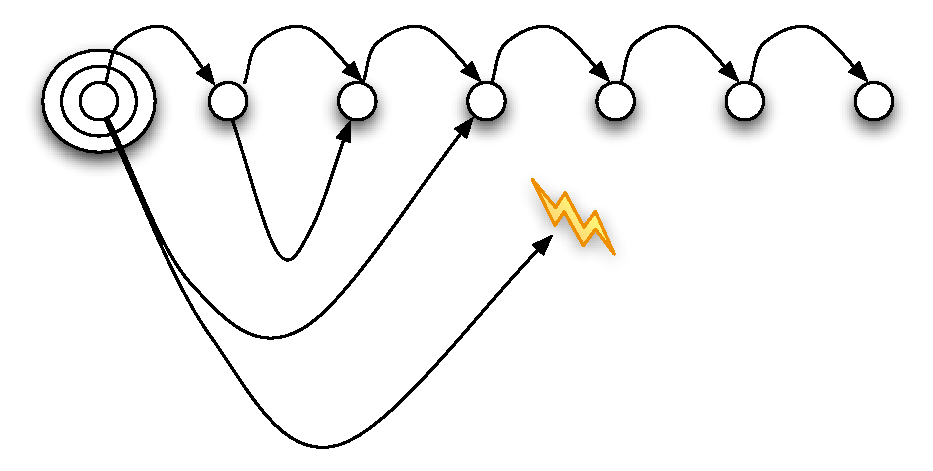
\includegraphics[width=0.75\linewidth]{dedalus-time.pdf}
  \label{fig:dedalus-time}
  \caption{Time moves forward in three ways: across strata, to the next fixpoint, and to some future fixpoint.}
\vspace{-8pt}
\end{figure}



